\documentclass[tikz,border=3.14pt]{standalone}

\usetikzlibrary{3d,decorations.text,shapes.arrows,positioning,fit,backgrounds,shapes.geometric,calc,decorations.markings,arrows}
\tikzset{pics/fake box/.style args={% #1=color, #2=x dimension, #3=y dimension, #4=z dimension
#1 with dimensions #2 and #3 and #4}{
code={
\draw[black,ultra thin,fill=#1]  (0,0,0) coordinate(-front-bottom-left) to
++ (0,#3,0) coordinate(-front-top-right) --++
(#2,0,0) coordinate(-front-top-right) --++ (0,-#3,0) 
coordinate(-front-bottom-right) -- cycle;
\draw[black,ultra thin,fill=#1] (0,#3,0)  --++ 
 (0,0,#4) coordinate(-back-top-left) --++ (#2,0,0) 
 coordinate(-back-top-right) --++ (0,0,-#4)  -- cycle;
\draw[black,ultra thin,fill=#1!80!black] (#2,0,0) --++ (0,0,#4) coordinate(-back-bottom-right)
--++ (0,#3,0) --++ (0,0,-#4) -- cycle;
\path[black,decorate,decoration={text effects along path,text={CONV}}] (#2/2,{2+(#3-2)/2},0) -- (#2/2,0,0);
}
}}
% from https://tex.stackexchange.com/a/52856/121799
\tikzset{circle dotted/.style={dash pattern=on .05mm off 2mm,
                                         line cap=round}}

\tikzset{%
  every neuron/.style={
    circle,
    draw,
    minimum size=0.6cm
  },
  neuron missing/.style={
    draw=none, 
    scale=4,
    text height=0.5cm,
    execute at begin node=\color{black}$\vdots$
  },
}


\begin{document}

\newsavebox\convarch


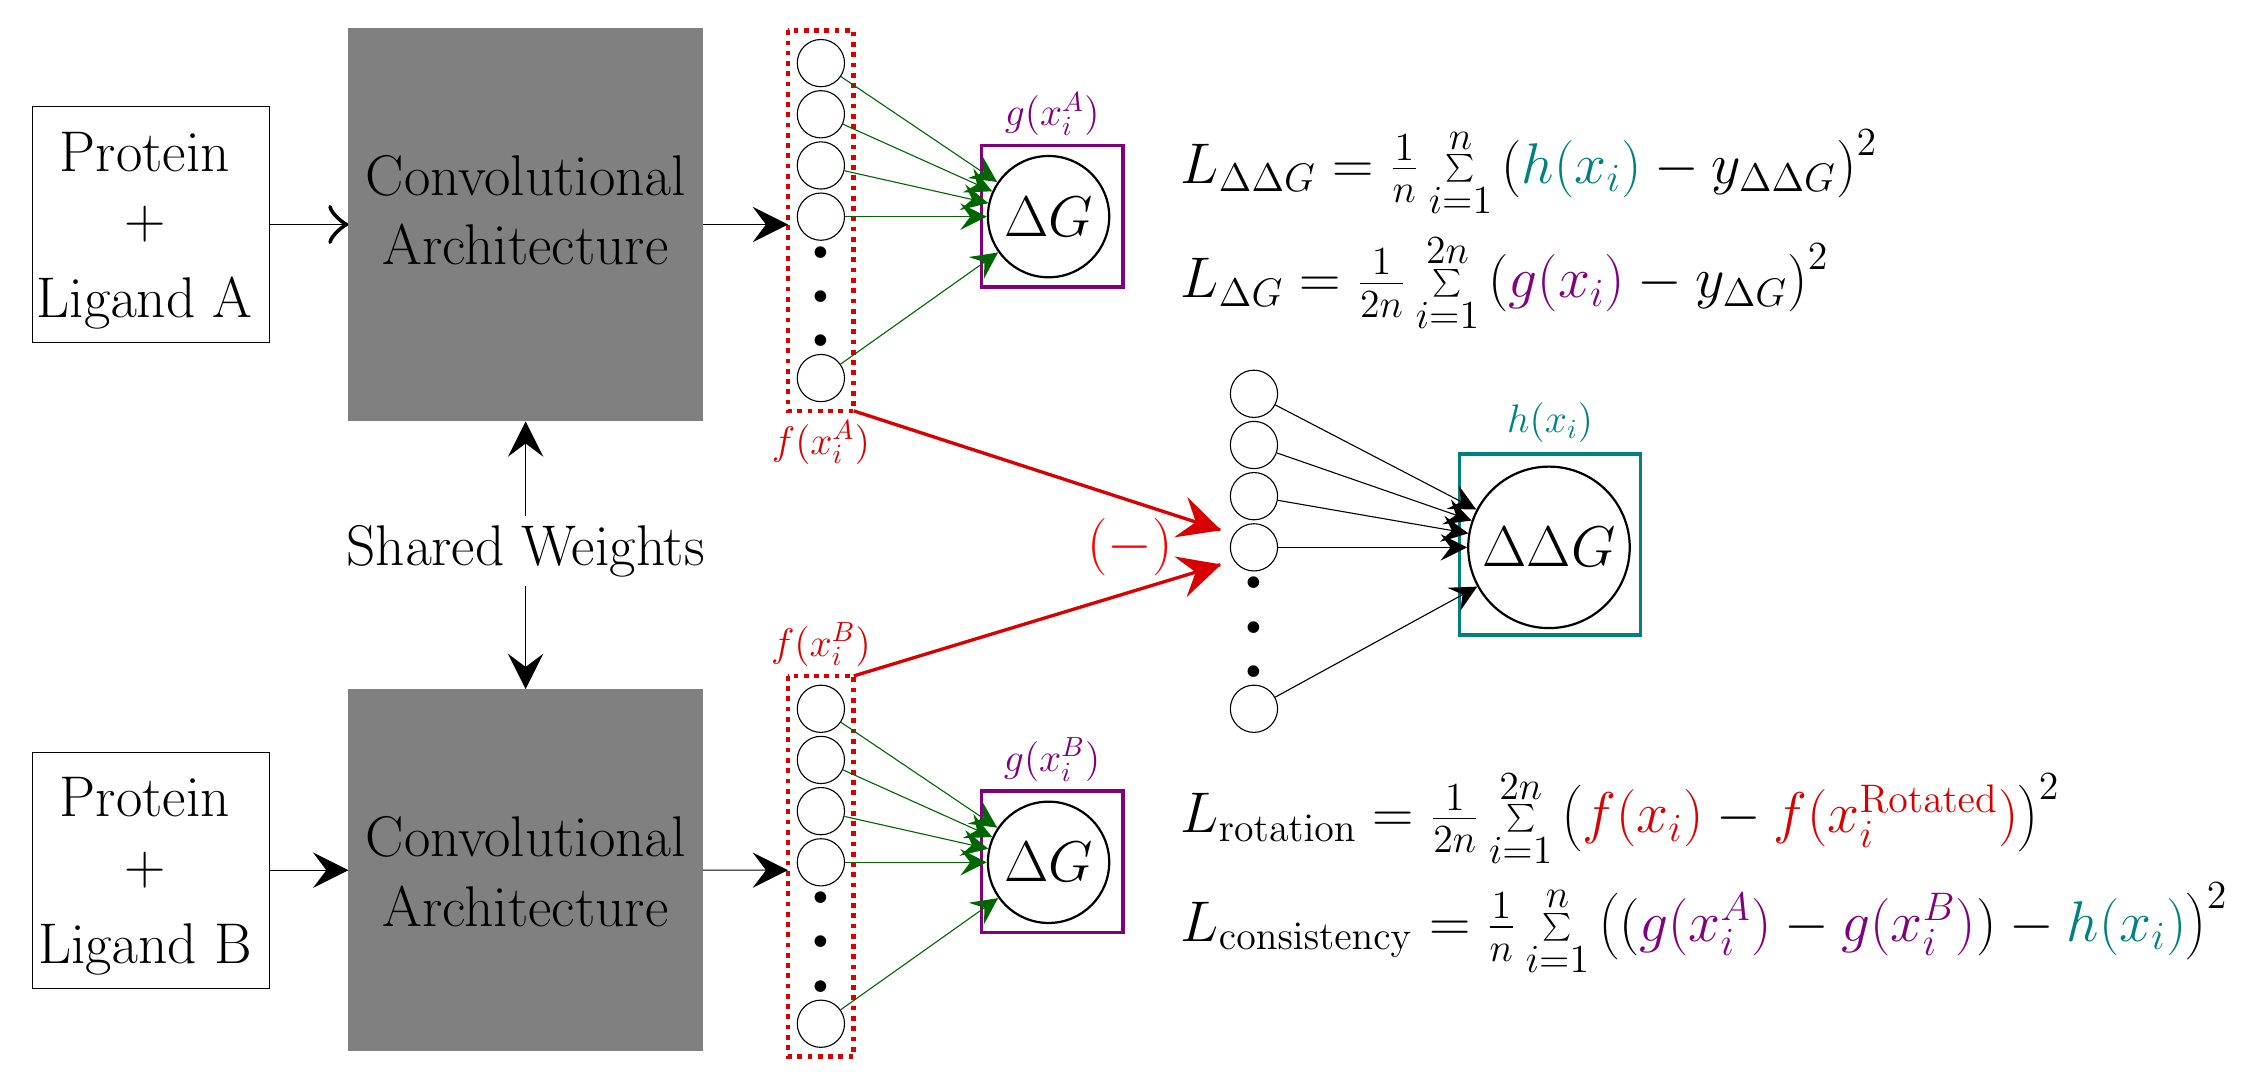
\begin{tikzpicture}        
        % Top Arm
                \begin{scope}[shift={(0,4)},x={(1,0)},y={(0,1)},z={({cos(60)},{sin(60)})},
                font=\sffamily\small,scale=2,local bounding box=calc1]
                %        \foreach \X [count=\Y] in {1.3,0.8,1.3,0.8,1.3}
                %        {
                %        \draw pic (box1-$\Y$) at (\Y,-\X/2,0) {fake box=white!70!gray with dimensions 0.75 and {2*\X} and 1*\X};
                %        }
                %        %
                       \scoped[on background layer]{
                        \fill[gray,thick] (0.75,-0.8) rectangle (3,1.7);}
                \end{scope}
        \node[font=\huge,below=1.5cm of calc1.north,align=center] (CNN) {Convolutional\\ Architecture};
        %inputs
	\node[font=\huge,left=2.2cm of calc1.west,anchor=east] (plus1) {$+$};
        \node[font=\huge,above=0.2cm of plus1] (prot1) {Protein};
        \node[font=\huge,below=0.2cm of plus1] (lig1) {Ligand A};
	\node[draw,minimum height=3cm,minimum width=3cm,left=of calc1.west,anchor=east] (togeth1) {}; 
	\draw[decoration={markings,mark=at position 1 with{\arrow[scale=4]{>}}},postaction={decorate},shorten >= 0.4pt] (togeth1.east) -- (calc1.west);

        %CNN output
        \foreach \m/\l [count=\y] in {1,2,3,4,missing}
                \node [every neuron/.try, neuron \m/.try] (flat1-\m) at ($(calc1.east)+(1.5cm,2.7cm-\y*0.65 cm)$) {};

        \foreach \m/\l [count=\y] in {5}
                \node [every neuron/.try, neuron \m/.try] (flat1-\m) at ($(calc1.east)+(1.5cm,-1.3cm-\y*0.65 cm)$) {};
        \draw[line width=0.6mm,black!15!red,dotted,local bounding box=flatten1] ($(flat1-1.north west)+(-0.2cm,0.2cm)$) rectangle ($(flat1-5.south east)+(0.2cm,-0.2cm)$);
        \draw[decoration={markings,mark=at position 1 with{\arrow[scale=4]{stealth}}},postaction={decorate},shorten >= 0.4pt] (calc1.east) -- ($(flatten1.west) + (0,-0.05cm)$);

        %dg calc
	% \node[font=\huge,rectangle,draw,fill=green!20,minimum height=2cm,minimum width=2cm,right=2cm of flatten1] (dg1) {h(x)}; 
        % \draw[decoration={markings,mark=at position 1 with{\arrow[scale=4]{stealth}}},postaction={decorate},shorten >= 0.4pt] (flatten1) -- (dg1); %arrows to subtract
        \node[font=\huge,draw,circle,thick,right=1.8cm of flat1-4] (aff1) {$\Delta G$};
        \draw[red!50!blue,very thick,local bounding box=aff1box] ($(aff1.north west) + (-0.3,0.35)$) rectangle ++(1.8,-1.8);
        \foreach \i in {1,...,5}
                \draw [black!60!green,decoration={markings,mark=at position 1 with{\arrow[scale=3]{stealth}}},postaction={decorate},shorten >= 0.4pt] (flat1-\i) -- (aff1);
        % \draw[decoration={markings,mark=at position 1 with{\arrow[scale=4]{stealth}}},postaction={decorate},shorten >= 0.4pt] (dg1) -- (aff1); %arrows to subtract

        %Bottom Arm
        \begin{scope}[shift={(0,-4)},x={(1,0)},y={(0,1)},z={({cos(60)},{sin(60)})},
        font=\sffamily\small,scale=2,local bounding box=calc2]
                %\foreach \X [count=\Y] in {1.3,0.8,1.3,0.8,1.3}
                %{
                %\draw pic (box1-$\Y$) at (\Y,-\X/2,0) {fake box=white!70!gray with dimensions 0.75 and {2*\X} and 1*\X};
                %}
                %%
                \scoped[on background layer]{
                \fill[gray,thick] (0.75,-0.8) rectangle (3,1.5);}
        \end{scope}
        \node[font=\huge,below=1.5cm of calc2.north,align=center] (CNN) {Convolutional\\ Architecture};
        % Inputs
	\node[font=\huge,left=2.2cm of calc2.west,anchor=east] (plus2) {$+$};
        \node[font=\huge,above=0.2cm of plus2] (prot2) {Protein};
        \node[font=\huge,below=0.2cm of plus2] (lig2) {Ligand B};
	\node[draw,minimum height=3cm,minimum width=3cm,left=of calc2.west,anchor=east] (togeth2) {}; 
	\draw[decoration={markings,mark=at position 1 with{\arrow[scale=4]{stealth}}},postaction={decorate},shorten >= 0.4pt] (togeth2.east) -- (calc2.west);

        %CNN output
        \foreach \m/\l [count=\y] in {1,2,3,4,missing}
                \node [every neuron/.try, neuron \m/.try] (flat2-\m) at ($(calc2.east)+(1.5cm,2.7cm-\y*0.65 cm)$) {};

        \foreach \m/\l [count=\y] in {5}
                \node [every neuron/.try, neuron \m/.try] (flat2-\m) at ($(calc2.east)+(1.5cm,-1.3cm-\y*0.65 cm)$) {};
        % \draw[fill=gray!50,local bounding box=flatten2] ($(calc2.east)+(1.2cm,-1.75cm)$) rectangle ++(0.4,4);
	% \draw[solid, black] ($(calc2.east)+(1.2cm,-1.75cm)$) grid [step=0.4cm] ++(0.4,4);
        \draw[line width=0.6mm,black!15!red,dotted,local bounding box=flatten2] ($(flat2-1.north west)+(-0.2cm,0.2cm)$) rectangle ($(flat2-5.south east)+(0.2cm,-0.2cm)$);
        \draw[decoration={markings,mark=at position 1 with{\arrow[scale=4]{stealth}}},postaction={decorate},shorten >= 0.4pt] (calc2.east) -- ($(flatten2.west) + (0,-0.05cm)$);

        %dg calc
	% \node[font=\huge,rectangle,draw,fill=green!20,minimum height=2cm,minimum width=2cm,right=2cm of flat2-5] (dg2) {h(x)}; 
        % \draw[decoration={markings,mark=at position 1 with{\arrow[scale=4]{stealth}}},postaction={decorate},shorten >= 0.4pt] (flat2-5) -- (dg2); %arrows to subtract
        \node[font=\huge,draw,circle,thick,right=1.8cm of flat2-4] (aff2) {$\Delta G$};
        \draw[red!50!blue,very thick,local bounding box=aff2box] ($(aff2.north west) + (-0.3,0.35)$) rectangle ++(1.8,-1.8);
        \foreach \i in {1,...,5}
                \draw [black!60!green,decoration={markings,mark=at position 1 with{\arrow[scale=3]{stealth}}},postaction={decorate},shorten >= 0.4pt] (flat2-\i) -- (aff2);
        % \draw[decoration={markings,mark=at position 1 with{\arrow[scale=4]{stealth}}},postaction={decorate},shorten >= 0.4pt] (dg2) -- (aff2); %arrows to subtract


        \foreach \m/\l [count=\y] in {1,2,3,4,missing}
                \node [every neuron/.try, neuron \m/.try] (sub-\m) at ($(calc1.east)+(7cm,-1.5cm-\y*0.65 cm)$) {};

        \foreach \m/\l [count=\y] in {5}
                \node [every neuron/.try, neuron \m/.try] (sub-\m) at ($(calc1.east)+(7cm,-5.5cm-\y*0.65 cm)$) {};

        % \draw[fill=gray!50,local bounding box=sub1] ($(calc1.east)+(4cm,-7.2cm)$) rectangle ++(0.4,4); %% subtraction
	% \draw[solid, black] ($(calc1.east)+(4cm,-7.2cm)$) grid [step=0.4cm] ++(0.4,4);
        \node[font=\huge,red,left=0.6cm of sub-4.west] (indicator) {$(-)$};
        \draw[black!15!red,very thick,decoration={markings,mark=at position 1 with{\arrow[scale=3]{stealth}}},postaction={decorate},shorten >= 0.4pt] (flatten1.south east) -- ($(sub-4.north west)-(0.2,0)$); %arrows to subtract
        \draw[black!15!red,very thick,decoration={markings,mark=at position 1 with{\arrow[scale=3]{stealth}}},postaction={decorate},shorten >= 0.4pt] (flatten2.north east) -- ($(sub-4.south west)-(0.2,0)$);

        \node[font=\huge,draw,circle,thick,right=2.4cm of sub-4] (final) {$\Delta\Delta G$};
        \draw[green!50!blue,very thick,local bounding box=finalbox] ($(final.north west) + (-0.4,0.45)$) rectangle ++(2.3,-2.3);
        \foreach \i in {1,...,5}
                \draw [decoration={markings,mark=at position 1 with{\arrow[scale=3]{stealth}}},postaction={decorate},shorten >= 0.4pt] (sub-\i) -- (final);

        %Extra Stuff
        \node[font=\huge,rectangle,below=1.2cm of calc1.south] (weights) {Shared Weights};
        \draw[decoration={markings,mark=at position 1 with{\arrow[scale=4]{stealth}}},postaction={decorate},shorten >= 0.4pt] (weights) -- (calc1.south); 
        \draw[decoration={markings,mark=at position 1 with{\arrow[scale=4]{stealth}}},postaction={decorate},shorten >= 0.4pt] (weights) -- (calc2.north); 

        %Loss Stuff
        %Boxes
        \node[font=\Large] (fA) at ($(flatten1.south)+(0,-0.4)$) {$\textcolor{black!15!red}{f(x_i^A)}$};
        \node[font=\Large] (fA) at ($(flatten2.north)+(0,0.4)$) {$\textcolor{black!15!red}{f(x_i^B)}$};
        \node[font=\Large] (gA) at ($(aff1box.north)+(0,0.4)$) {$\textcolor{red!50!blue}{g(x_i^A)}$};
        \node[font=\Large] (gB) at ($(aff2box.north)+(0,0.4)$) {$\textcolor{red!50!blue}{g(x_i^B)}$};
        \node[font=\Large] (h) at ($(finalbox.north)+(0,0.4)$) {$\textcolor{green!50!blue}{h(x_i)}$};

        \node[font=\huge,anchor=west] (ddg_loss) at ($(aff1.north east) + (1cm,0)$) {$L_{\Delta\Delta G}=\frac{1}{n}\sum\limits_{i=1}^{n}\left(\textcolor{green!50!blue}{h(x_i)}-y_{\Delta\Delta G}\right)^2$};
        \node[font=\huge,anchor=west] (dg_loss) at ($(aff1.north east) + (1cm,-1.4cm)$) {$L_{\Delta G}=\frac{1}{2n}\sum\limits_{i=1}^{2n}\left(\textcolor{red!50!blue}{g(x_i)}-y_{\Delta G}\right)^2$};

        \node[font=\huge,anchor=west] (rot_loss) at ($(aff2.north east) + (1cm,0)$) {$L_{\mathrm{rotation}}=\frac{1}{2n}\sum\limits_{i=1}^{2n}\left(\textcolor{black!15!red}{f(x_i)}-\textcolor{black!15!red}{f(x_{i}^{\mathrm{Rotated}})}\right)^2$};
        \node[font=\huge,anchor=west] (cons_loss)  at ($(aff2.north east) + (1cm,-1.4cm)$) {$L_{\mathrm{consistency}}=\frac{1}{n}\sum\limits_{i=1}^{n}\left((\textcolor{red!50!blue}{g(x_i^A)}-\textcolor{red!50!blue}{g(x_i^B)})-\textcolor{green!50!blue}{h(x_i)}\right)^2$};
        
\end{tikzpicture}           
\end{document}
